\begin{figure}[!t]
\centering
\begin{tikzpicture}[scale=0.85]

% TRANSFORMER ARCHITECTURE
\draw[fill=gray_bbox_color, line width=0.046875cm, rounded corners=0.300000cm] (-0.975000, 6.455000) -- (2.725000, 6.455000) -- (2.725000, 1.305000) -- (-0.975000, 1.305000) -- cycle;

\draw[line width=0.046875cm, fill=emb_color, rounded corners=0.100000cm] (0.000000, 0.000000) -- (2.500000, 0.000000) -- (2.500000, -0.900000) -- (0.000000, -0.900000) -- cycle;
\node[text width=2.500000cm, align=center] at (1.250000,-0.450000) {\footnotesize Trajectory \vspace{-0.3cm} \linebreak Embedding};
\draw[line width=0.046875cm, fill=add_norm_color, rounded corners=0.100000cm] (0.000000, 3.680000) -- (2.500000, 3.680000) -- (2.500000, 3.180000) -- (0.000000, 3.180000) -- cycle;
\node[text width=2.500000cm, align=center] at (1.250000,3.430000) {\footnotesize Add \& Norm};
\draw[line width=0.046875cm, fill=multi_head_attention_color, rounded corners=0.100000cm] (0.000000, 3.030000) -- (2.500000, 3.030000) -- (2.500000, 2.130000) -- (0.000000, 2.130000) -- cycle;
\node[text width=2.500000cm, align=center] at (1.250000,2.580000) {\footnotesize Multi-Head \vspace{-0.3cm} \linebreak Attention};
\draw[line width=0.046875cm] (1.250000, 3.030000) -- (1.250000, 3.180000);
\draw[line width=0.046875cm, fill=add_norm_color, rounded corners=0.100000cm] (0.000000, 6.230000) -- (2.500000, 6.230000) -- (2.500000, 5.730000) -- (0.000000, 5.730000) -- cycle;
\node[text width=2.500000cm, align=center] at (1.250000,5.980000) {\footnotesize Add \& Norm};
\draw[line width=0.046875cm, fill=ff_color, rounded corners=0.100000cm] (0.000000, 5.580000) -- (2.500000, 5.580000) -- (2.500000, 4.680000) -- (0.000000, 4.680000) -- cycle;
\node[text width=2.500000cm, align=center] at (1.250000,5.130000) {\footnotesize Feed \vspace{-0.3cm} \linebreak Forward};
\draw[line width=0.046875cm] (1.250000, 0.600000) circle (0.200000);
\draw[line width=0.046875cm] (1.410000, 0.600000) -- (1.090000, 0.600000);
\draw[line width=0.046875cm] (1.250000, 0.760000) -- (1.250000, 0.440000);
\draw[line width=0.046875cm] (0.350000, 0.600000) circle (0.400000);
\draw[line width=0.046875cm] (-0.030000, 0.600000) -- (-0.014490, 0.629156) -- (0.001020, 0.657833) -- (0.016531, 0.685561) -- (0.032041, 0.711884) -- (0.047551, 0.736369) -- (0.063061, 0.758616) -- (0.078571, 0.778258) -- (0.094082, 0.794973) -- (0.109592, 0.808486) -- (0.125102, 0.818576) -- (0.140612, 0.825077) -- (0.156122, 0.827883) -- (0.171633, 0.826946) -- (0.187143, 0.822284) -- (0.202653, 0.813971) -- (0.218163, 0.802145) -- (0.233673, 0.786999) -- (0.249184, 0.768783) -- (0.264694, 0.747796) -- (0.280204, 0.724382) -- (0.295714, 0.698925) -- (0.311224, 0.671845) -- (0.326735, 0.643584) -- (0.342245, 0.614608) -- (0.357755, 0.585392) -- (0.373265, 0.556416) -- (0.388776, 0.528155) -- (0.404286, 0.501075) -- (0.419796, 0.475618) -- (0.435306, 0.452204) -- (0.450816, 0.431217) -- (0.466327, 0.413001) -- (0.481837, 0.397855) -- (0.497347, 0.386029) -- (0.512857, 0.377716) -- (0.528367, 0.373054) -- (0.543878, 0.372117) -- (0.559388, 0.374923) -- (0.574898, 0.381424) -- (0.590408, 0.391514) -- (0.605918, 0.405027) -- (0.621429, 0.421742) -- (0.636939, 0.441384) -- (0.652449, 0.463631) -- (0.667959, 0.488116) -- (0.683469, 0.514439) -- (0.698980, 0.542167) -- (0.714490, 0.570844) -- (0.730000, 0.600000);
\draw[line width=0.046875cm, -latex] (1.250000, 3.680000) -- (1.250000, 4.680000);
\draw[line width=0.046875cm, -latex] (1.250000, 0.000000) -- (1.250000, 0.400000);
\draw[line width=0.046875cm, -latex] (1.250000, 0.800000) -- (1.250000, 2.130000);
\draw[line width=0.046875cm] (0.750000, 0.600000) -- (1.050000, 0.600000);
\draw[-latex, line width=0.046875cm, rounded corners=0.200000cm] (1.250000, 4.080000) -- (-0.750000, 4.080000) -- (-0.750000, 5.980000) -- (0.000000, 5.980000);
\draw[-latex, line width=0.046875cm, rounded corners=0.200000cm] (1.250000, 1.530000) -- (-0.750000, 1.530000) -- (-0.750000, 3.430000) -- (0.000000, 3.430000);
\draw[-latex, line width=0.046875cm, rounded corners=0.200000cm] (1.250000, 1.730000) -- (0.312500, 1.730000) -- (0.312500, 2.130000);
\draw[-latex, line width=0.046875cm, rounded corners=0.200000cm] (1.250000, 1.730000) -- (2.187500, 1.730000) -- (2.187500, 2.130000);
\draw[line width=0.046875cm, -latex] (1.250000, -1.500000) -- (1.250000, -0.900000);
\node[text width=2.500000cm, anchor=north, align=center] at (1.250000,-1.500000) {\footnotesize Agent \vspace{-0.3cm} \linebreak Trajectories};
\node[anchor=east] at (-1.175000,3.880000) {$4 \times$};
\node[anchor=east] at (-1.175000,9.68) {$|\Upsilon| \times$};
\node[text width=2.000000cm, anchor=east] at (0.250000,0.600000) {\footnotesize Positional \vspace{-0.3cm} \linebreak Encoding};

%----------------------------------------------------------------------------------------------------------------------------
% CONVOLUTIONAL ARCHITECTURE
\draw[fill=gray_bbox_color, line width=0.046875cm, rounded corners=0.300000cm] (3.775000, 10.155) -- (7.475000, 10.155) -- (7.475000, 1.305000) -- (3.775000, 1.305000) -- cycle;


\draw[line width=0.046875cm, fill=conv_color, rounded corners=0.1cm] (4, 2.03) -- (6.5, 2.03) -- (6.5, 1.53) -- (4, 1.53) -- cycle;
\node[text width=2.500000cm, align=center] at (5.25, 1.83) {\footnotesize \vspace{-0.15cm} $\text{Conv}_{2 \times 16}$};
\draw[line width=0.046875cm] (5.250000, 2.03) -- (5.250000, 2.18);
\draw[line width=0.046875cm, fill=pool_color, rounded corners=0.1cm] (4, 2.68) -- (6.5, 2.68) -- (6.5, 2.18) -- (4, 2.18) -- cycle;
\node[text width=2.500000cm, align=center] at (5.25, 2.48) {\footnotesize \vspace{-0.15cm} MaxPool};

\draw[line width=0.046875cm, -latex] (5.250000, 2.68) -- (5.250000, 3.18);

\draw[line width=0.046875cm, fill=conv_color, rounded corners=0.1cm] (4, 3.68) -- (6.5, 3.68) -- (6.5, 3.18) -- (4, 3.18) -- cycle;
\node[text width=2.500000cm, align=center] at (5.25, 3.48) {\footnotesize \vspace{-0.15cm} $\text{Conv}_{16 \times 32}$};
\draw[line width=0.046875cm] (5.250000, 3.68) -- (5.250000, 3.83);
\draw[line width=0.046875cm, fill=conv_color, rounded corners=0.1cm] (4, 4.33) -- (6.5, 4.33) -- (6.5, 3.83) -- (4, 3.83) -- cycle;
\node[text width=2.500000cm, align=center] at (5.25, 4.13) {\footnotesize \vspace{-0.15cm} $\text{Conv}_{32 \times 32}$};

\draw[line width=0.046875cm, -latex] (5.250000, 4.33) -- (5.250000, 4.83);

\draw[line width=0.046875cm, fill=conv_color, rounded corners=0.1cm] (4, 5.33) -- (6.5, 5.33) -- (6.5, 4.83) -- (4, 4.83) -- cycle;
\node[text width=2.500000cm, align=center] at (5.25, 5.13) {\footnotesize \vspace{-0.15cm} $\text{Conv}_{32 \times 64}$};
\draw[line width=0.046875cm] (5.250000, 5.33) -- (5.250000, 5.48);
\draw[line width=0.046875cm, fill=conv_color, rounded corners=0.1cm] (4, 5.98) -- (6.5, 5.98) -- (6.5, 5.48) -- (4, 5.48) -- cycle;
\node[text width=2.500000cm, align=center] at (5.25, 5.78) {\footnotesize \vspace{-0.15cm} $\text{Conv}_{64 \times 64}$};

\draw[line width=0.046875cm, -latex] (5.250000, 5.98) -- (5.250000, 6.48);

\draw[line width=0.046875cm, fill=conv_color, rounded corners=0.1cm] (4, 6.98) -- (6.5, 6.98) -- (6.5, 6.48) -- (4, 6.48) -- cycle;
\node[text width=2.500000cm, align=center] at (5.25, 6.78) {\footnotesize \vspace{-0.15cm} $\text{Conv}_{64 \times 128}$};
\draw[line width=0.046875cm] (5.250000, 6.98) -- (5.250000, 7.13);
\draw[line width=0.046875cm, fill=conv_color, rounded corners=0.1cm] (4, 7.63) -- (6.5, 7.63) -- (6.5, 7.13) -- (4, 7.13) -- cycle;
\node[text width=2.500000cm, align=center] at (5.25, 7.43) {\footnotesize \vspace{-0.15cm} $\text{Conv}_{128 \times 128}$};

\draw[line width=0.046875cm, -latex] (5.250000, 7.63) -- (5.250000, 8.13);

\draw[line width=0.046875cm, fill=pool_color, rounded corners=0.1cm] (4, 8.63) -- (6.5, 8.63) -- (6.5, 8.13) -- (4, 8.13) -- cycle;
\node[text width=2.500000cm, align=center] at (5.25, 8.43) {\footnotesize \vspace{-0.15cm} AvgPool};
\draw[line width=0.046875cm] (5.250000, 8.63) -- (5.250000, 8.78);
\draw[line width=0.046875cm, fill=conv_color, rounded corners=0.1cm] (4, 9.28) -- (6.5, 9.28) -- (6.5, 8.78) -- (4, 8.78) -- cycle;
\node[text width=2.500000cm, align=center] at (5.25, 9.08) {\footnotesize \vspace{-0.15cm} $\text{Conv}_{128 \times 256}$};
\draw[line width=0.046875cm] (5.250000, 9.28) -- (5.250000, 9.43);
\draw[line width=0.046875cm, fill=conv_color, rounded corners=0.1cm] (4, 9.93) -- (6.5, 9.93) -- (6.5, 9.43) -- (4, 9.43) -- cycle;
\node[text width=2.500000cm, align=center] at (5.25, 9.73) {\footnotesize \vspace{-0.15cm} $\text{Conv}_{256 \times 128}$};


\draw[-latex, line width=0.046875cm, rounded corners=0.200000cm] (5.25, 2.78) -- (7.25, 2.78) -- (7.25, 4.48) -- (5.25, 4.48);
\draw[-latex, line width=0.046875cm, rounded corners=0.200000cm] (5.25, 4.63) -- (7.25, 4.63) -- (7.25, 6.13) -- (5.25, 6.13);
\draw[-latex, line width=0.046875cm, rounded corners=0.200000cm] (5.25, 6.28) -- (7.25, 6.28) -- (7.25, 7.78) -- (5.25, 7.78);

\node[anchor=west] at (7.675000,5.7300) {$1 \times$};
\node[text width=2.500000cm, align=center] at (5.250000,-0.450000) {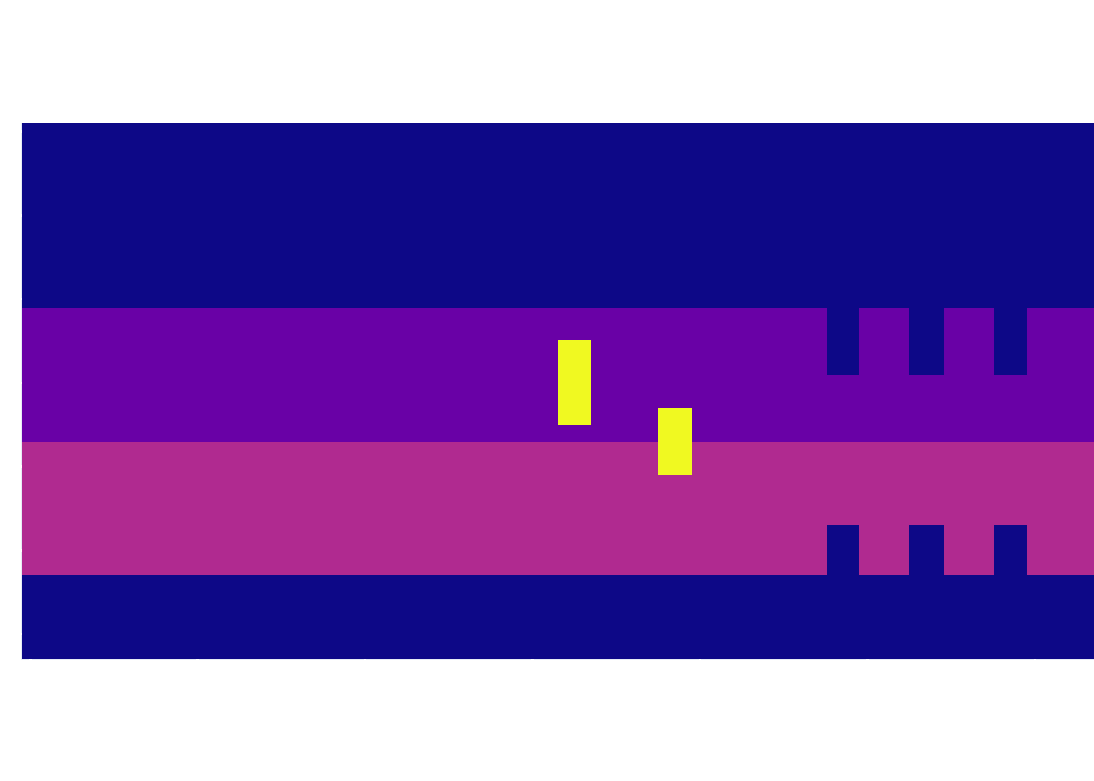
\includegraphics[scale=0.15]{images/agent_view.pdf}};
\draw[line width=0.046875cm, -latex] (5.250000, 0.35) -- (5.250000, 1.53);

%--------------------------------------------------------------------------------------------------------------------------------------------
% Policy Network
\draw[line width=0.046875cm, fill=ff_color, rounded corners=0.100000cm] (0.000000, 10.08) -- (2.500000, 10.08) -- (2.500000, 9.18) -- (0.000000, 9.18) -- cycle;
\node[text width=2.500000cm, align=center] at (1.250000, 9.68) {\footnotesize Policy \vspace{-0.3cm} \linebreak Network};

\node[text width=2.500000cm, align=center] at (0.312500, 11.580000) {$\bm \mu$};
\node[text width=2.500000cm, align=center] at (1.250000, 11.580000) {$\bm \sigma$};
\node[text width=2.500000cm, align=center] at (2.187500, 11.580000) {$ \hat V$};

\draw[-latex, line width=0.046875cm, rounded corners=0.200000cm] (1.250000, 10.730000) -- (0.312500, 10.730000) -- (0.312500, 11.33);
\draw[-latex, line width=0.046875cm, rounded corners=0.200000cm] (1.250000, 10.730000) -- (2.187500, 10.730000) -- (2.187500, 11.33);
\draw[line width=0.046875cm, -latex] (1.250000, 10.03) -- (1.250000, 11.33);

\draw[line width=0.046875cm, -latex] (1.250000, 6.230000) -- (1.250000, 9.23);
\draw[line width=0.046875cm, -latex] (4, 9.68) -- (2.5, 9.68);

\end{tikzpicture}
\caption[Multi-agent Transformer]{The Transformer model used in this thesis. On the right side, an ECA-ResNet processes visual input maps and outputs a vector representation. On the left side, the states of all agents $\Upsilon$ relative to the ego-agent are embedded and then fed into a Transformer encoder. The resulting $|\Upsilon|$ vectors are concatenated with the output of the convolutional pipeline. A parameter-shared \gls{mlp} policy decodes the concatenated representations, producing a distribution $(\bm \mu, \bm \sigma)$ and a value estimate $\hat V$ for each agent.}\label{fig:transformer}
\end{figure}